\documentclass[10pt,twocolumn,letterpaper]{article}

\usepackage{cvpr}
\usepackage{times}
\usepackage{booktabs}
\usepackage{indentfirst}
\usepackage{epsfig}
\usepackage{float}
\usepackage{amsmath}
\usepackage{picinpar,graphicx}
\usepackage[breaklinks=true,bookmarks=false,colorlinks,
            linkcolor=red,
            anchorcolor=blue,
            citecolor=green,
            backref=page]{hyperref}

\cvprfinalcopy % *** Uncomment this line for the final submission
\def\cvprPaperID{****} % *** Enter the CVPR Paper ID here
\def\httilde{\mbox{\tt\raisebox{-.5ex}{\symbol{126}}}}


\begin{document}

%%%%%%%%% TITLE
\title{Discriminative Region Proposal AdversarialNetworks for High-Quality Image-to-Image Translation}

\author{Wenjie Niu\\\\ July 19,2018}

\maketitle
After several days of reading the paper of Discriminative Region Proposal Adversarial Networks for High-Quality Image-to-Image Translation, I have access to the framework, structure and basic professional knowledge such as Convolutional Neural Network(CNN) and Generative Adversarial Network(GAN). However, there are some difficulties for me like the deprivation of formula in the understanding of GAN. \par
\begin{abstract}
In this paper, authors present Discrimitive Rigion Proposal Adversarial Network(DRPAN) for high-quality image-to-image translation. In order to reduce the artifacts and blur problems during the process of translation, they explore the patch discriminator.  It produces the score map and find the most artificial part by a sliding window. Then put the discriminitive region mask the coresponding real image to obtain a fake-mask real image. A reviser based on GANs is used to distinguish the real to fake-mask real to help improving the translation quality.
\end{abstract}

\section{Introducion}
The procedure of image-to-image translation task is descomposed into three iterated steps. First is to generate a fake image with some local artifacts by generator. Second is to propose the most fake region from the genrated image using DRPnet as shown in figure.~\ref{fig:DRPnet}. Third is to mask real image with the discriminative region, so that DPRAN(as shown in figure.~\ref{fig:DRPAN}) can optimazed on the most fake part.\par
There are three main contribution in this paper:
\begin{itemize}
\item discriminators based on patch for producing discriminative region;
\item reviser based on GANs to provide constructive revisions for generator
\item building a DRPAN model
\end{itemize}

\begin{figure*}
\begin{center}
   \includegraphics[width=1\linewidth]{DRPnet.png}
\end{center}
   \caption{\textbf{Left}: Their Discriminative Region Proposal network (DRPnet). \textbf{Right}: Synthesized samples compared with previous works on Cityscapes validation dataset~\cite{Cordts2016The}. The regions within red window show obvious artifacts or deformation. Their method can synthesize images with clear structure and vivid details.~\cite{Wang2017Discriminative}}
\label{fig:DRPnet}
\end{figure*}

\begin{figure*}
\begin{center}
   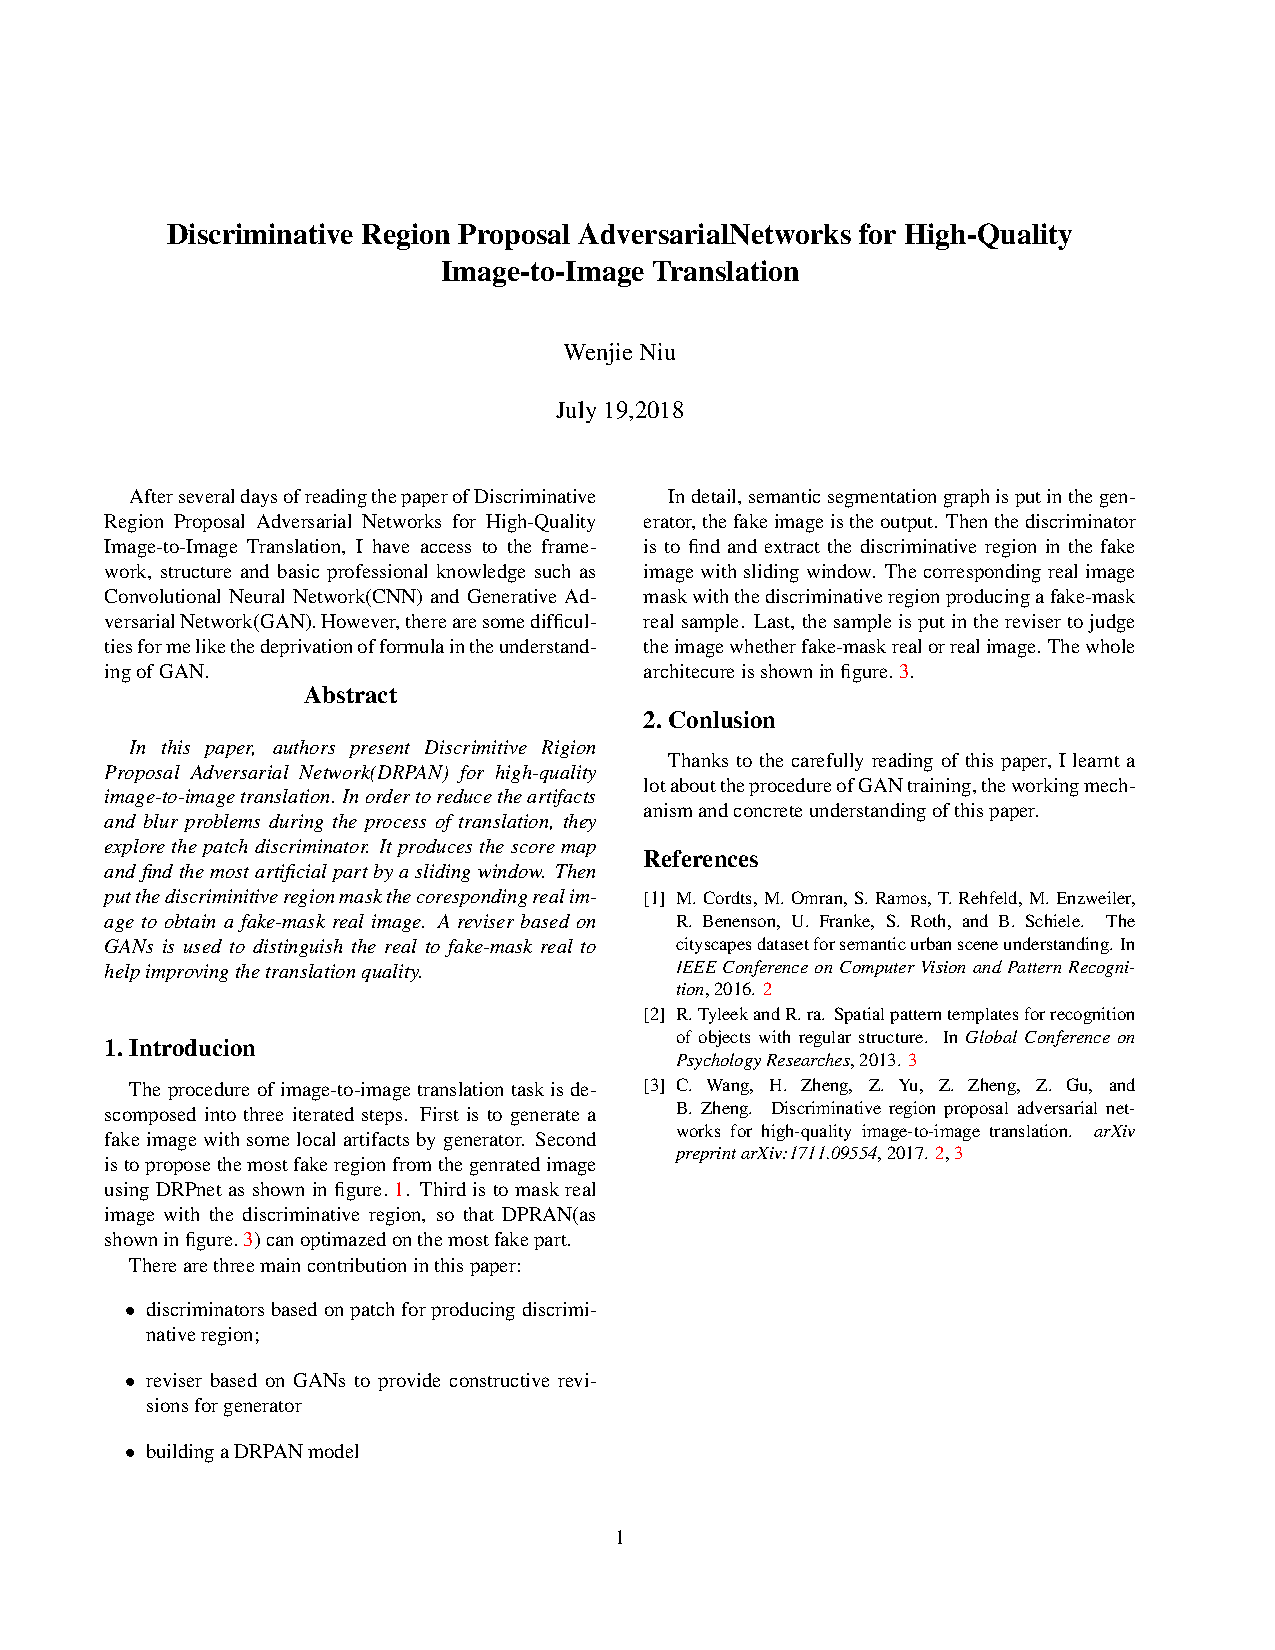
\includegraphics[width=1\linewidth]{DRPAN.png}
\end{center}
   \caption{The overall network architecture and data flow of our proposed Discriminative Region Proposal Adversarial Network (DRPAN), which is composed of three components: a generator, a discriminator, and a reviser, and is a unified model for image-to-image translation tasks.~\cite{Wang2017Discriminative}}
\label{fig:DRPAN}
\end{figure*}

In detail, semantic segmentation graph is put in the generator, the fake image is the output. Then the discriminator is to find and extract the discriminative region in the fake image with sliding window. The corresponding real image mask with the discriminative region producing a fake-mask real sample. Last, the sample is put in the reviser to judge the image whether fake-mask real or real image. The whole architecure is shown in figure.~\ref{fig:DRPAN}.

\begin{figure*}
\begin{center}
   \includegraphics[width=1\linewidth]{facades.png}
\end{center}
   \caption{The training process of DRPAN on facades dataset~\cite{Radim2013Spatial}. Left: The plotting curve shows mean value of score map on synthesized samples. Right: Step by step synthesis on different discriminative regions.~\cite{Wang2017Discriminative}}
\label{fig:Process}
\end{figure*}


\section{Method}
Figure.~\ref{fig:Process} shows the process of how to improve the quality of synthesized image. With DRPAN's training, the discriminative of fake-mask real image  varies improving the quality of synthesized image and scoring higher. 

\begin{figure*}
\begin{center}
   \includegraphics[width=1\linewidth]{PatchGAN.png}
\end{center}
   \caption{The output results of score map on different quality levels (fake and real) of images by a pre-trained PatchGAN. The darkest regions on score maps mean the lowest quality, indicating that patch-based discriminators can be explored for discriminative region proposal.~\cite{Wang2017Discriminative}}
\label{fig:PatchGAN}
\end{figure*}

Figure.~\ref{fig:PatchGAN} shows the output results of score map on different quality levels(fake and real) of images by a pre-trained PatchGAN. The score maps of the fake samples are almost dark with lower score while of the real samples are brightest with highest scores.\par
Given an input image with resolution $w_i \times w_i$, and processed by the patch discriminator to be a probability score map with size $w_s \times w_s$. Suppose we want to obtain the discriminative region at $w^* \times w^*$, the size of sliding window $w$ for score map can be calculated by
\begin{equation}
w=w^* \times w_s/w_i
\end{equation}
Then our DRPnet will find the discriminative square patch on score map with the center coordinates $(x_c,y_c)$ and length $w$, so the scale$\tau$ between the input image and output score map is
\begin{equation}
\tau=\frac{w_i-w^*}{w_s-w}
\end{equation}
The center coordinates $(x_c^*,y_c^*)$ of discriminative region will be calculated by
\begin{equation}
\begin{cases}
x_c^*=\tau\times x_c,\\
y_c^*=\tau\times y_c.
\end{cases}
\end{equation}
Finally, the discriminative region d r produced by DRPnet can be expressed as
\begin{equation}
d_r=F_{DRPnet}(x_c^*,y_c^*,w^*)
\end{equation}


\section{Conlusion}
Thanks to the carefully reading of this paper, I learnt a lot about the procedure of GAN training, the working mechanism and concrete understanding of this paper. There are quite some difficulty in the understanding of the equations, I still need some time to catch.
%-------------------------------------------------------------------------

{\small
\bibliographystyle{ieee}
\bibliography{DRPAN}
}

\end{document}
